%% LyX 2.1.4 created this file.  For more info, see http://www.lyx.org/.
%% Do not edit unless you really know what you are doing.
\documentclass[11pt,czech,american]{book}
\usepackage[T1]{fontenc}
\usepackage[utf8]{inputenc}
\usepackage[a4paper]{geometry}
\geometry{verbose,tmargin=4cm,bmargin=3cm,lmargin=3cm,rmargin=2cm,headheight=0.8cm,headsep=1cm,footskip=0.5cm}
\pagestyle{headings}
\setcounter{secnumdepth}{3}
\usepackage{url}
\usepackage{amsmath}
\usepackage{amsthm}
\usepackage{amssymb}
\usepackage{graphicx}
\usepackage{setspace}
\usepackage[final]{pdfpages}
\usepackage{natbib}
\usepackage{mathrsfs}
\usepackage{algorithm}
\usepackage{algorithmicx}
\usepackage[noend]{algpseudocode}
\usepackage{caption}


\usepackage{array}
\usepackage{ragged2e}

\usepackage{lipsum}
\usepackage{psvectorian}

\DeclareMathOperator*{\argmax}{arg\,max}

\makeatletter
%%%%%%%%%%%%%%%%%%%%%%%%%%%%%% Textclass specific LaTeX commands.
\newenvironment{lyxlist}[1]
{\begin{list}{}
{\settowidth{\labelwidth}{#1}
 \setlength{\leftmargin}{\labelwidth}
 \addtolength{\leftmargin}{\labelsep}
 \renewcommand{\makelabel}[1]{##1\hfil}}}
{\end{list}}

%%%%%%%%%%%%%%%%%%%%%%%%%%%%%% User specified LaTeX commands.
%% Font setup: please leave the LyX font settings all set to 'default'
%% if you want to use any of these packages:

%% Use Times New Roman font for text and Belleek font for math
%% Please make sure that the 'esint' package is turned off in the
%% 'Math options' page.
\usepackage[varg]{txfonts}

%% Use Utopia text with Fourier-GUTenberg math
%\usepackage{fourier}

%% Bitstream Charter text with Math Design math
%\usepackage[charter]{mathdesign}

%%---------------------------------------------------------------------

%% Make the multiline figure/table captions indent so that the second
%% line "hangs" right below the first one.
%\usepackage[format=hang]{caption}

%% Indent even the first paragraph in each section
\usepackage{indentfirst}

%%---------------------------------------------------------------------

%% Disable page numbers in the TOC. LOF, LOT (TOC automatically
%% adds \thispagestyle{chapter} if not overriden
%\addtocontents{toc}{\protect\thispagestyle{empty}}
%\addtocontents{lof}{\protect\thispagestyle{empty}}
%\addtocontents{lot}{\protect\thispagestyle{empty}}

%% Shifts the top line of the TOC (not the title) 1cm upwards 
%% so that the whole TOC fits on 1 page. Additional page size
%% adjustment is performed at the point where the TOC
%% is inserted.
%\addtocontents{toc}{\protect\vspace{-1cm}}

%%---------------------------------------------------------------------

% completely avoid orphans (first lines of a new paragraph on the bottom of a page)
\clubpenalty=9500

% completely avoid widows (last lines of paragraph on a new page)
\widowpenalty=9500

% disable hyphenation of acronyms
\hyphenation{CDFA HARDI HiPPIES IKEM InterTrack MEGIDDO MIMD MPFA DICOM ASCLEPIOS MedInria}

%%---------------------------------------------------------------------

%% Print out all vectors in bold type instead of printing an arrow above them
\renewcommand{\vec}[1]{\boldsymbol{#1}}

% Replace standard \cite by the parenthetical variant \citep
%\renewcommand{\cite}{\citep}

\makeatother

\usepackage{babel}

\newcommand{\ornamentleft}{%
	\psvectorian[width=2em]{2}%
}
\newcommand{\ornamentright}{%
	\psvectorian[width=2em,mirror]{2}%
}

\newcommand{\ornamentheader}[1]{%
	\begin{center}
		\ornamentleft
		\quad{\large\emph{#1}}\quad % style as desired
		\ornamentright
	\end{center}%
}

\newlength{\rlength}\setlength{\rlength}{16cm}
\newcommand{\ruletext}[2][\rlength]{%
	\noindent%
	\parbox{#1}{%
		\noindent\dotfill\raisebox{-.3\ht\strutbox}{#2}\dotfill\par}%
}





\begin{document}
\def\documentdate{July 7, 2017}

\newtheorem{definition}{Definition}[chapter]
\newtheorem{note}{Note}[chapter]
\newtheorem{example}{Example} 
\newtheorem{assumption}{Assumption} 

\newtheorem{theorem}{Theorem}
\newtheorem*{remark}{Remark}

\captionsetup[figure]{labelfont={bf},labelformat={default},labelsep=period,name={Fig.}}


\def\documentdate{\today}

\pagestyle{empty}
{\centering

\noindent %
\begin{minipage}[c]{3cm}%
\noindent \begin{center}

\includegraphics[width=3cm,height=3cm,keepaspectratio]{Images/TITLE/cvut}
\par\end{center}%
\end{minipage}%
\begin{minipage}[c]{0.6\linewidth}%
\begin{center}
\textsc{\large{}Czech Technical University in Prague}{\large{}}\\
{\large{}Faculty of Nuclear Sciences and Physical Engineering}
\par\end{center}%
\end{minipage}%
\begin{minipage}[c]{3cm}%
\noindent \begin{center}

\includegraphics[width=3cm,height=3cm,keepaspectratio]{Images/TITLE/fjfi}
\par\end{center}%
\end{minipage}

\vspace{3cm}


\textbf{\huge{}Real Options Valuation: A Dynamic Programming Approach}{\huge \par}

\vspace{1cm}


\selectlanguage{czech}%
\textbf{\huge{}Oceňování projektů metodou reálných opcí z pohledu dynamického progamování}{\huge \par}

\selectlanguage{american}%
\vspace{2cm}


{\large{}Master's Thesis}{\large \par}

}

\vfill{}

\begin{lyxlist}{MMMMMMMMM}
\begin{singlespace}
\item [{Author:}] \textbf{Filip Rolenec}
\item [{Supervisor:}] \textbf{Ing. Rudolf Kulhavý, DrSc.}
\end{singlespace}

\item [{Language~advisor:}] \textbf{Ing. Rudolf Kulhavý, DrSc.} 
\begin{singlespace}
\item [{Academic~year:}] 2020/2021\end{singlespace}

\end{lyxlist}
\newpage{}

~\newpage{}

~

\vfill{}


\begin{center}
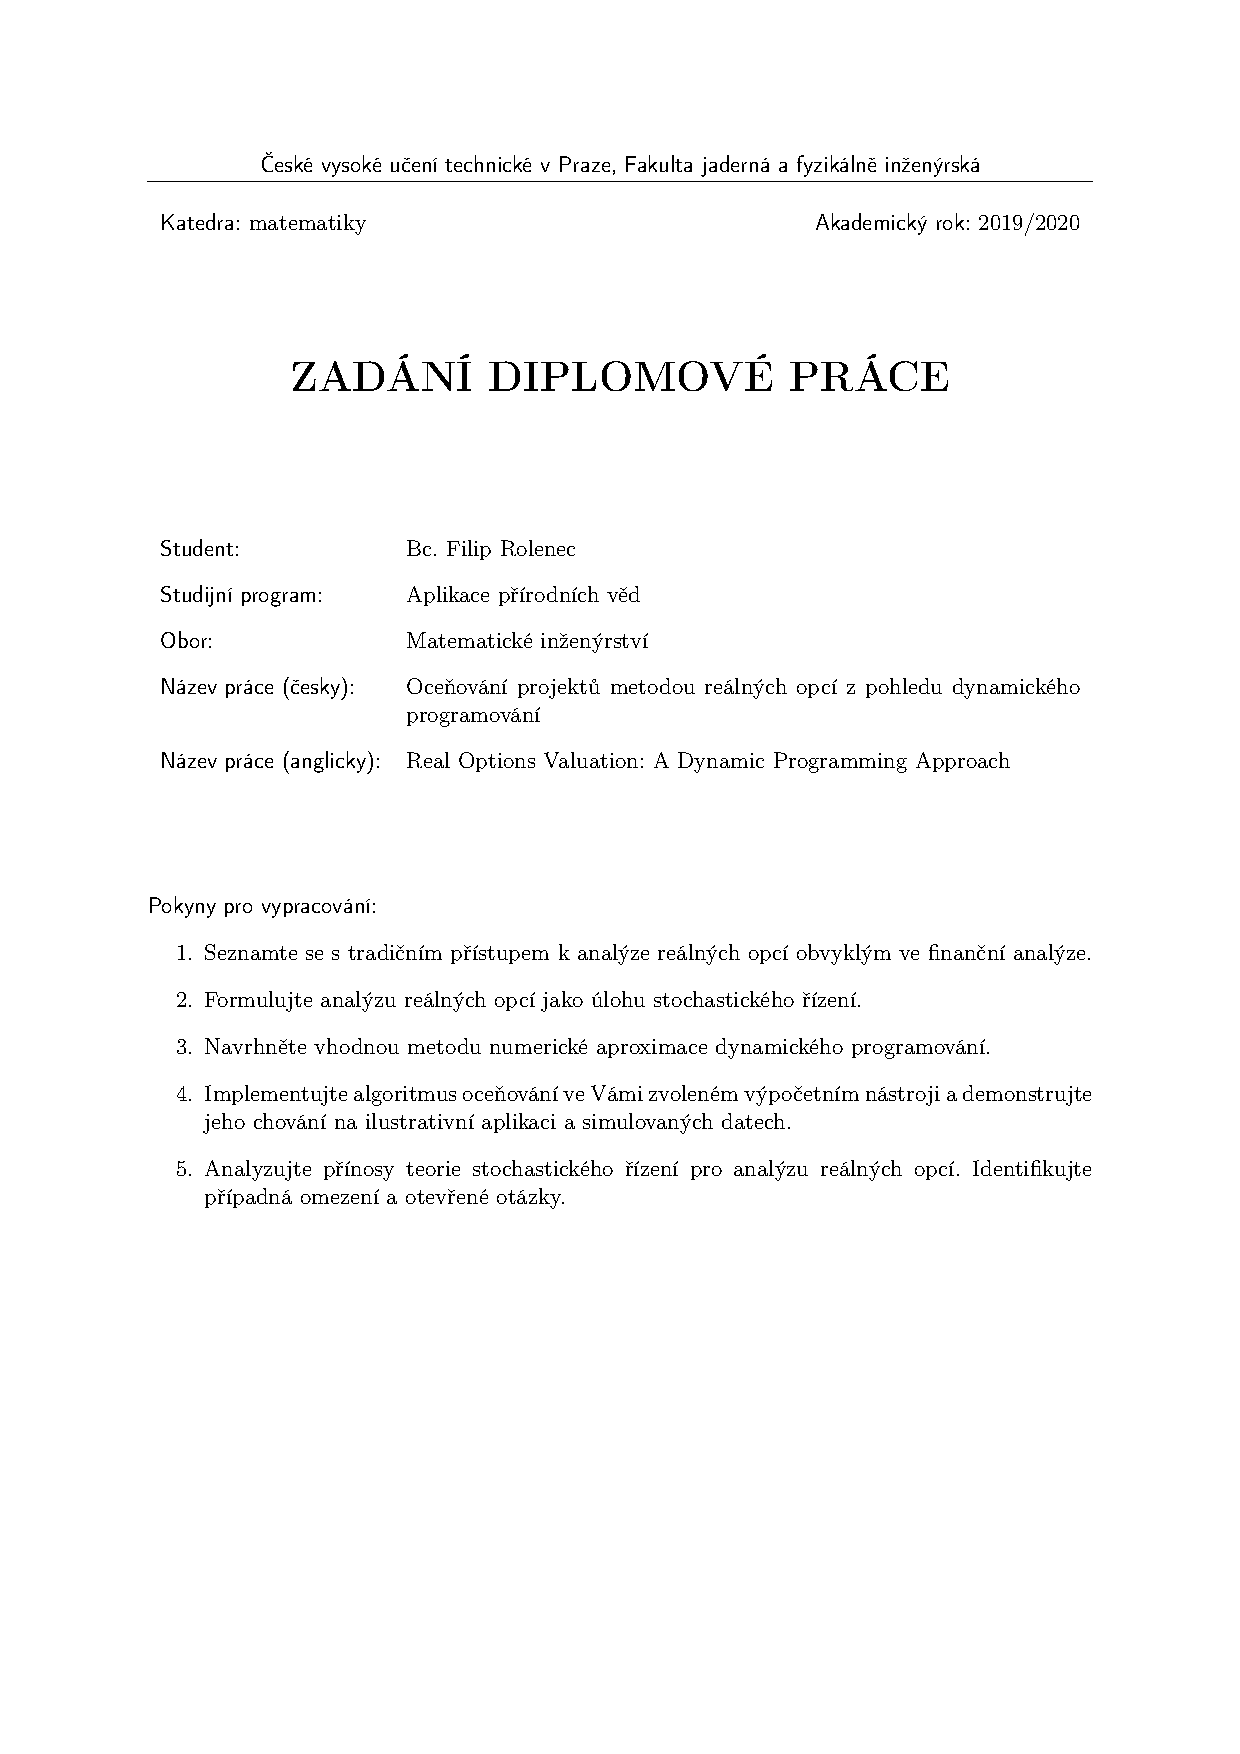
\includepdf[pages={1}]{Images/zadaniMT.pdf}


\par\end{center}

\vfill{}


~\newpage{}

~

\vfill{}


\begin{center}
\includepdf[pages={2}]{Images/zadaniMT.pdf}
\par\end{center}

\vfill{}


~\newpage{}

\noindent \emph{\Large{}Acknowledgment:}{\Large \par}

\noindent I would like to thank my supervisor Ing. Rudolf Kulhavý, DrSc. for his professional guidance and all the advice given while creating this thesis. 

\vfill

\noindent \emph{\Large{}Author's declaration:}{\Large \par}

\noindent I declare that this Master's thesis is entirely
my own work and I have listed all the used sources in the bibliography.

\bigskip{}


\noindent Prague, \documentdate\hfill{}Bc. Filip Rolenec

\vspace{2cm}


\newpage{}

~\newpage{}

\selectlanguage{czech}%
\begin{onehalfspace}
\noindent \emph{Název práce:}

\noindent \textbf{Oceňování projektů metodou reálných opcí z pohledu dynamického progamování}
\end{onehalfspace}

\bigskip{}


\noindent \emph{Autor:} Bc. Filip Rolenec

\bigskip{}


\noindent \emph{Obor:} Matematické inženýrství 


\bigskip{}


\noindent \emph{Druh práce:} Diplomová práce

\bigskip{}


\noindent \emph{Vedoucí práce:} Ing. Rudolf Kulhavý, DrSc.


\bigskip{}


\noindent \emph{Abstrakt:} \textbf{BUDE DOPLNĚNO }


\bigskip{}


\noindent \emph{Klíčová slova:}   Analýza reálných opcí, Blackův-Scholesův model, Čistá současná hodnota, Dynamické programování, Energetika, Oceňování projektů, Stochastická rozhodovací teorie



\selectlanguage{american}%
\vfill{}
~

\begin{onehalfspace}
\noindent \emph{Title:}

\noindent \textbf{Real Options Valuation: A Dynamic Programming Approach}
\end{onehalfspace}

\bigskip{}


\noindent \emph{Author:} Bc. Filip Rolenec

\bigskip{}


\noindent \emph{Abstract:} \textbf{WILL BE ADDED}
	
	
\bigskip{}


\noindent \emph{Keywords:} Black-Scholes model, Dynamic programming, Net present value, Power industry, Project valuation,  Real option analysis, Stochastic decision control

\newpage{}

~\newpage{}

\pagestyle{plain}

\tableofcontents{}

\newpage{}


\chapter{Historical background and research motivation}
The foundations of financial derivatives date back to the origins of commerce in Mesopotamia in the fourth millennium BC \cite{Web:09}. The derivative market consisted mainly of forward contracts \footnote{A forward contract is a contract to purchase an asset at a fixed price on a particular date in the future. \cite{BerDeM:09} } and it was introduced to the European continent through Spain in Roman times. After the expulsion of derivative trading in Spain the center of this type of commerce for Europe were the Low Lands. There, in the end of the 17th century, the first ideas about options \footnote{A financial option is the \textbf{ability} to buy (call option) or sell (put option) a defined volume of an asset for a defined amount of money in a given future time instant. \cite{BerDeM:09}}  and option trading are published by La Vega \cite{Veg:88}. 

The first attempts of a mathematical option pricing come from Bachelier (1900) \cite{Bac:00} and Bronzin  (1908) \cite{Bro:08}. Based on their work the boom of option pricing methods in the 1970's culminated by Nobel-price-winning Black-Scholes model \cite{BlaSch:73}, which is today's standard in the option pricing theory\cite{YalHak:12}. 

The publicity and wide adoption of the BSM model most likely inspired an expert on capital budgeting, Stewart Myers, to introduce the term "Real Options" \cite{Mye:77}, which is one of two main pillars of this thesis. Myers builds on the idea that part of the project's value is hidden in the form of real options - ability to change the course of the project in the future. Myers' approach to the real options is mostly philosophical in a sense that he stresses the importance of thinking about the additional value options bring, while he does not present any computational tool for the said value. 

The idea of Real Option Analysis (ROA) as a valuation tool for projects was further developed by several influential authors in the following decades, for example Guthrie \cite{Gut:09}, Vollert \cite{Vol:03} Pindyck \cite{DixPin:12} and Kulatilaka \cite{AmrKul:98}. 

The valuation of project's free cash flows with the theory of ROA is in the economical world understood as very advanced and its adoption in practice is slow \cite{Amp:17}. It is argued that this slow adoption is caused mainly by misunderstanding the more difficult mathematical concept of ROA \cite{SicGam:10} and the low adoption rate of a competition: "Why should our company use a new tool that no one else is using?" \cite{CopAnt:01}. 

Through the study of the ROA state of the art, we have identified that there is a discrepancy in understanding what ROA actually is. As will be illustrated in depth in section ... we identify three classes of ROA authors based on the level of analogy to the BSM model. 

In this thesis we focus on the second class of ROA authors represented by brilliant publications of Graeme Guthrie \cite{Gut:09} and Alexander Vollert \cite{Vol:03}.\footnote{Second class utilizes only the no-arbitrage principle to determine probabilities of the models.}  

Through my studies at the FNSPE CTU, I have specialized in the theory of dynamic decision making under uncertainty \cite{Rol:18}, \cite{Rol:19}. When studying ROA it came only natural to understand the project valuation as an optimal decision making problem. 

The goal of this thesis is to take the project valuation problem structure as is understood in ROA and look at it from the perspective of stochastic decision theory (SDT). One of the challenges of this task is to implement domain specific economical truths about the behavior of investors and the way they perceive value.  Two main addressed concepts are: the time value of money and the risk-aversion of investors. 

The goal of this thesis is to provide an SDT-based valuation algorithm for projects, whose value is understood as a maximal possible current cash equivalent of the uncertain future cash flows. This valuation algorithm will cover the classes of problems now solved by ROA and allow for new classes. 

The new SDT based valuation algorithm will enable: 
\begin{itemize}
	\item seamless integration of multiple uncertainty sources;
	\item integration of theoretically any probability distribution as a model of uncertain variables;
	\item usage of high number of possible actions, regardless of their nature; 
	\item utilization of approximate dynamic programming tools for high-dimensional problems;
	\item preservation the economical truths as time value of money and the risk-aversion of investors. 
\end{itemize}

To illustrate the usage of the new SDT-based algorithm a valuation of a project from a selected class is performed. This class is denoted as \textit{facilities with simple input-output process models}. It covers all projects whose cycle time is equal zero and the input-output transformation rate is constant. This class is a generalization motivated by an example of gas power plant valuation presented by Guthrie in \cite{Gut:09}. 


The thesis is structured in 5 chapters. Chapter 1 reminds the reader of the most important mathematical and economical concepts used in this thesis. Beginning with the declaration of mathematical notation the chapter continues with key concepts of economical theory and deeper description of the BSM model. The first chapter continues with a summary of the last decades in ROA research with the focus on a specific level of analogy represented by Vollert \cite{Vol:03} and Guthrie \cite{Gut:09}. The reminder of the first chapter is reserved for key parts of stochastic decision theory. 

Chapter 2 represents the core of this thesis. First, we define what will be understood as a problem of ROA project valuation. We state the key features that define a project and we limit this features accordingly (?). Then we focus on the interpretation of the problem by a general SDT framework. We illustrate the identification of ROA project features in SDT. The reminder of the  second chapter is reserved for resolving the economical nuances that need to be accounted for in the SDT framework in order to make the valuation procedure consistent with the economical reality of investors' behavior. 

Chapter 3 illustrates the new valuation algorithm from chapter 2 on an example of valuation of a facility with a simple input-output process model. A valuation of a gas power plant is chosen as the representative of this class. The first half of the chapter focuses on the value sensitivity with regard to the volume of available managerial actions in the project. The second half presents a value comparison  of project alternations in different granularity of the model structure and it is aimed to demonstrate the existence of trade-of between computational complexity and precision of computed results. 

Chapter 4 discusses the new findings both theoretical and observed from the performed experiments. 

Chapter 5 summarizes the thesis - reminds the motivation, underlines the main message and lists all contributions of this thesis. Furthermore, it outlines many possible future research paths in this field as it is, to our best knowledge, the first available publication on this topic. 


%\addcontentsline{toc}{chapter}{Introduction}

%\addcontentsline{toc}{chapter}{Preliminaries}

\pagestyle{headings}




\chapter{Preliminaries}
\ruletext{Introduction to preliminaries}

To properly understand a mathematical text it is important to first define the used notions and symbolism. Since this thesis is based on many different authors, from both financial and mathematical world, a short unifying overview of the used theory is important. 

The notation used in this thesis comes predominantly from the most influential authors in the respective fields of study: 
\begin{itemize}
	\item general economy \cite{BerDeM:09};
	\item real options \cite{Gut:09};
	\item stochastic decision theory \cite{BacChi:19}.
\end{itemize}

 The pure mathematical symbolism comes from the author's studying experience at FNSPE CTU and its applicability is proven in his previous works \cite{Rol:18} and \cite{Rol:19}. 


\ruletext{}
\section{Used mathematical symbolism}
\ruletext{Sets, random variables, what do I mean by 'probability'}

In the whole thesis, bold capital letters, such as $\mathbf{X}$, represent a set of all elements $x \in \mathbf{X}$ as in \cite{Rol:18}. The cardinality of a set $\mathbf{X}$ is denoted with two vertical lines as $|\mathbf{X}|$. Random variables, understood in a sense of the standard Kolmogorov's probability theory \cite{Kol:60}\footnote{Does this citation make sense?}, are represented with a tilde above the variable, i.e. $\tilde{x}$. Realizations of random variables are denoted by the same letters as the random variable without the tilde, i.e. $x$. 

\begin{definition}(Probability)
	Let $\tilde{x}$ be a random discrete variable. Then $P(x)$ denotes a probability that the realization of $\tilde{x}=x$. Similarly if $\tilde{x}$ is a continuous random variable, then $p(x)$ denotes a probability density of the realization $\tilde{x}=x$. 
\end{definition}
\begin{remark}
	To rigorously unify the notation and simplify the formulas a Radon-Nikodým (RN) density \cite{Rao:87a} is introduced  with the notation $p(x)$ and the name ``probability density``. The dominating measure of this RN density is either the counting measure (in discrete case) or the Lebesgue measure (in continuous case). The notation $P(X)$ is reserved only for the cases when the discreteness of the argument needs to be emphasized. 
\end{remark}

The last general definition is the definition of well known concept of conditional probability \cite{Jay:03}. 
\begin{definition}(Conditional probability)
	Let, depending on the context, symbol $p(x|y)$ represents either the conditional probability on discrete variables or the conditional probability density on continuous variables. Then the $p(x|y)$ is defined as:
	\begin{equation}\label{eq:condP}
	p(x|y)=\frac{p(x,y)}{p(y)},
	\end{equation} where $p(x,y)$ is a joint probability density of $x$ and $y$. 
\end{definition}

\begin{remark}
	The definition of conditional probability expressed by the equation (\ref{eq:condP}) corresponds with the classic definitions of the conditional probability and conditional probability density in both the discrete and continuous case. 
\end{remark}

<Probably some other definitions that will be needed in the following chapters> 

\ruletext{}

\section{General economics}
\ruletext{Introduction and basic financial concepts. }

This thesis is built on two main theoretical pillars, the theory of corporate finance \cite{BerDeM:09} and stochastic decision theory (SDT) \cite{BacChi:19}. A basic review of corporate finance terminology is presented in this section with a focus on project valuation techniques. 


\begin{definition}(Project)
	A project is defined as a piece of planned work or an activity that is finished over a period of time and intended to achieve a particular purpose, mainly a wealth increase of a company or an individual. \footnote{First part comes from Cambridge dictionary. Is that ok just to cite it? }
\end{definition}

\begin{definition}(Value)
	The amount of money that can be received for something. \footnote{Again cambridge dictionary...Find a better definition of value. } 
\end{definition}

<The value of project is created by elementary monetary transactions in time> 

<Tracking each individual transaction is impractical, thus the models work by aggregation in time, or with the continuous notion> 

<We will use the discrete aggregation over time periods> 

<There are multiple metric in economics that try to describe the financial flows in a company. In this thesis we will use FCF (defined as in Berk DeMarzo, look at it in detail), since it fits best the notion of value in time> 

<We will understand FCF as being aggregated over time> 

\begin{definition}(Free cash flow)
	The incremental effect of a project on the firm’s available cash is the project’s free cash flow \cite{BerDeM:09}.
\end{definition}


\ruletext{}

\subsection{Net present value and other valuation metrics}
\ruletext{NPV, DTA, IRR, WACC and others}
<Say that this section is for illustration of current state of thinking about investments> 

<Say that NPV is the standard in this field> 

<Define NPV and say it is for illustration purposes> 

<A short paragraph about other metrics used in the decision making about a project, DTA,  IRR, WACC> 

\subsection{Risk averse investors}
<There is a correlation between the volatility of an investment and its average profits> 

<This is being explained by the risk-averse investors> 

<The risk-aversion is a known phenomenon studied also by psychology [find article to cite]sim>


\subsection{Option valuation - Black-Scholes-Merton model}

<The story of the motivation for BSM model is in the first chapter, reference it> 

<Here we will look at the details mathematical rigorous definition> 

<Plus author's view, what the theorem actually states (expected value of price)> 


Only four parameters and one assumption is needed to determine a value of an option according to BSM model for option pricing. Assume that the market is complete, and thus the law of one price holds \cite{}. Then to value a option you need to know only its time to maturity, its strike price, the current price of the underlying stock and its volatility as follows \cite{BerDeM:09}: 
\begin{equation}
C = SN(d_1) - PV(K)N(d_2), 
\label{BSMModelEq}
\end{equation}
where $S$ is the strike price, $PV(K)$ is a price of a bond paying K on the expiration day of the option and $N(d)$ is a cumulative normal distribution, probability that a normally distributed variable is less than $d$. Value of $d_1$ and $d_2$ is then defined as: 
\begin{equation}
d_1 = \frac{ln(S/PV(K))}{\sigma \sqrt{T}}+\frac{\sigma \sqrt{T}}{2}
d_2 = d_1 - \sigma \sqrt{T}
\end{equation}

The dependency of the price of an option is positive in case of volatility and time to maturity Increasing these parameters leads to a higher option price. On the contrary the rise in current stock price or strike price of the options lowers the value of an option. 




\section{Real option analysis}\label{sec:ROA}

<ROA originates as an analogy to financial option valuation> 

<There are three classes of authors using this term> 

<Full analogy paragraph> 

<Effective market analogy paragraph> 

<No analogy paragraph> 

This established and well received technique for financial option valuation spawned the idea of real option analysis. The option to buy an asset for a given price is similar to the ability to buy an expected future cash flow, i.e. invest in a project. 

<Origins of real options> The first economist, pioneer of the term \textit{Real option analysis}, ... ... treats investments as a complete analogy of trading with options. To be able to delay an investment has a value and..... 

The usage of the phrase real option analysis in literature is rather fuzzy. It is used by many authors such as \cite{BerDeM:09}, \cite{Gut:09} and \cite{Gue:17}, however their usage of the term differs. Three different usage classes of the term real option analysis were identified by the author. They differ by the level of analogy to the valuation of financial options. 

\paragraph{Complete analogy}
First, there is a class of complete analogy. All five parameters of financial options needed for their valuation with BSM model are identified with the parameters of an investment opportunity. An example of a valuation of a car dealership can be found in \cite{BerDeM:09}\footnote{Should I reference page numbers? Will anybody actually look up the example? } where the following identification is made:

\begin{table}[H]
	\begin{footnotesize}
		
		\centering
		\renewcommand{\arraystretch}{1,2}
		\label{Tab:BSModel}
			\begin{tabular}{|l |r|}
			\hline	
			Financial option& Real option \\ \hline
			Stock price& Current market value of asset \\ \hline
			Strike price& Upfront investment required	\\ \hline
			Expiration date& Final decision date \\ \hline
			Risk-free rate& Risk-free rate\\ \hline
			Volatility of stock & Volatility of asset value \\ \hline
			Dividend & FCF lost from delay \\ \hline
			
		\end{tabular}
		\caption{Identification of parameters for real options with respect to the financial option \cite{BerDeM:09}. }
	\end{footnotesize}
\end{table}

Another example can be found in \cite{Que:10} where a telecommunication company is being valued by the complete analogy valuation technique. 

This class of authors focuses on the clear analogy and thus the acknowledged scope of possible manager's actions is limited basically only to timing options. The only decision is to invest to a project now or later.


\paragraph{Partial analogy}

The second class of authors uses only the core property of the financial analogy and that is the law-of-one-price. With the help of this assumption, the authors, eg. \cite{Gut:09} usually derive risk-neutral probabilities which are then used for modeling of some internal variable of the cash flow functions. 

This class of authors is the most numerous and most mathematically rigorous. The core of publications in this class is usually in solving stochastic differential equations, eg. \cite{Vol:03} whereas the role of the assumption about law-of-one-price is used mainly as the ground for obtaining one of the missing parameters of the stochastic model. 

\paragraph{No analogy}

Third class of authors does not use the law-of-one-price and is thus the farthest away from the original idea of ....\footnote{The pioneer name}. This class of authors, i.e. \cite{Kas:04} and \cite{Gue:17}, understands the term real option analysis as a useful lens for looking at the project valuation. They accentuate the value of further managerial decision, but the valuation structure and algorithms do not differ from the DTA approach as defined earlier. 

Thus, this class of authors is declared as a misuse of terminology and not further considered. 

\bigskip

In the next part of the thesis, namely \ref{} the core message behind the term real option analysis will be thoroughly discussed. 

\ruletext{}

\section{Statistical decision theory}
\ruletext{Standard SDT as a framework, states, actions, inputs, outputs, rewards, probability distributions}

The second pillar upon which this thesis stands is the statistical decision theory (SDT). An area of applied mathematics that formalizes and studies optimal decision making of agents. As decision making in its broadest sense encapsulates a vast amount of human behavior, the class of problems it is able to solve is quite large. 

The SDT's main focus is to determine the optimal strategy (a sequence of decisions) to act upon, generally in dynamic and uncertain environment. A classical structure of a decision making problem consists of five building blocks

\begin{itemize}
	\item Set of time epochs - $\mathbf{T}$;
	\item Set of environment states in those epochs - $\mathbf{S}$;\footnote{Possibly different $S_t$ in different times.}
	\item Set of actions in those states - $\mathbf{A}$;
	\item Reward function of transition from one state to another - $r(s_t|a_t,s_{t-1})$;
	\item Transition probabilities governing the transitions from one state to another $p(s_t|a_t,s_{t-1})$.
\end{itemize}

The set of time epochs, states, actions is usually known, defined by the structure of the decision problem that is being solved. Reward and transition functions tend to be unknown in solving these problems and they need to be often somehow estimated. 

Usually, the biggest task in SDT is to correctly approach the uncertainty about transition probabilities between the different states of a project. There are two approaches to parameter estimation in statistics, classical approach and a Bayesian approach. Since the Bayesian approach seems to fit the format of decision making better - allowing for smooth updating on newly observed data - it is used in this thesis. 

The goal of SDT is to find the optimal strategy - sequence of actions. The optimality of such strategy is defined as it having the maximal expected cumulative reward among all eligible strategies 

\begin{equation}
	\pi^*=\argmax_{\pi \in \mathbf{\Pi}} E\left[\sum_{t\in \mathbf{T}} r(s_t|a_t,s_{t-1})|\pi\right].
\end{equation}

This maximization can be in total absolute values (in finite or discounted cases) or per time period (mostly in infinite non-discount cases). Due to the economic nature of this thesis we will focus on the total cumulative reward of a finite process (?). 

\subsection{Dynamic programming}
To maximize over all possible strategies by computing the expected cumulative reward for each one of them is a very demanding task even for low-dimensional decision problems. 

Thus, a clever idea of backward induction called dynamic programming is used. A function, called the value function is defined on the set of all possible states $\mathbf{S}$. This function represents the expected cumulative reward to be obtained from the given state onwards. The idea of backward induction is based on the truth that a sequence of actions is optimal if and only if the last action is optimal. 

This clever computation of value functions from the problem horizon backwards through all the possible states of the problem decreases the complexity from exponential to polynomial. Instead of maximizing over $|\mathbf{A}|^{|\mathbf{S|^{\mathbf{|T|}}}}$ possible strategies at once, one needs to compute significantly less demanding complexity of $|\mathbf{A}|\cdot|\mathbf{T}|\cdot{|\mathbf{S}|}$. \footnote{Check this}

The formula representing the backward induction is called the Bellman equation: 

\begin{equation}
	V(s_{t-1}) = \sum_{s_t \in \mathbf{S_t}} p(s_t|a_t, s_{t-1}) [r(s_t|a_t, s_{t-1})+V(s_t)].
\end{equation}

By defining the value function on the horizon, we can compute value functions of states with lower and lower time indexes, until we get to the time 0, which represents the present. Not only that we have the expected value of the optimal decision making, but we have also derived the optimal strategy for every possible path through the state space. 

The backward induction reduces the computation complexity significantly. However, for even a moderate-dimensional decision problems, the number of computations is still extremely large. 

The problem of computational complexity of dynamic programming is called "three curses of dimensionality" \cite{Pow:11} and various solutions have been proposed. These solutions are as a group referenced as approximate dynamic programming. 


\subsection{Approximate dynamic programming}

The computational complexity of dynamic programming for moderate and high-dimensional decision making problems is so demanding that results cannot be obtained in a reasonable amount of time. 

The response to this problem comes in a form of approximate dynamic programming, a section of decision making under uncertainty, that is represented by a number of algorithms that are trying to obtain quasi-optimal strategies with more reasonable demand for computation power. 

There are many different algorithms, that try to obtain approximate results of the precise dynamic programming represented by the bellman equation. In this thesis the ADP algorithm called <Q-learning, SARSA...> is used because of its high performance in ..., while being still relatively easy to implement. A longer discussion of its choice is left to its corresponding chapter \ref{}. 

\paragraph{<Q-Learning, SARSA,..>}
<Detailed description of the chosen ADP algorithm> 


\subsection{Bayesian statistics}

The field of mathematical statistics can be divided into two branches, classical (also called frequentist) and Bayesian. The philosophies of each one are fundamentally different, however in principle, they can serve for revealing new truths of the measured data in a similar fashion. 

Mathematical statistics is a very broad topic, not possible to summarize it in one paragraph. The use of Bayesian statistics in this thesis is only as a tool, no broader discussions about the internal philosophy of different approaches are presented.

In general, statistical theory is used to determine a distribution from which the observed data come from. In majority of cases, it is assumed that the data are realizations of a random variable with a distribution from some parameterized class - normal, log-normal, poisson, etc. The goal is then to determine, with some level of confidence, the parameters that fit the observed data in some sense the best. \footnote{Large simplification, statistics can be used in many different ways.} 

The main difference between the Bayesian and classical statistics is how the parameters of a distribution are perceived by the statistician. In the classical theory, it is assumed that observed data come from some distribution with some firm but unknown parameters $\Theta$. In contrast, the Bayesian view on the parameters is such that they are perceived as random variables $\tilde{\Theta}$. 

This terminology twist can be a source of initial confusion for frequentist statisticians, but it allows a simple and elegant update of parameter estimates with the Bayes formula.

\begin{equation}
	p(\Theta|d)=\frac{p(d|\Theta)p(\Theta)}{p(d)}, 
\end{equation}
where $\Theta$ is generally a multivariate parameter and $d$ are observed data. \footnote{The p(d) in denominator needs to be rewritten as integral if this formula is really to be used.}

The interpretation of Bayes formula, is that the distribution of parameter $p(\Theta)$ called the prior distribution, is updated for the newly observed data $d$, providing new, posterior,  distribution $p(\Theta|d)$. 

This update can be understood as learning about the "true value" of a parameter, which is very useful structure for dynamic decision problems. 

Since the Bayesian theory tells us only how to update an already existing distribution, a prior distribution needs to be given, even though no data were measured yet. 

This problem is in Bayesian statistics understood as an advantage, since one can use his knowledge about the problem that is being solved and incorporate it to the prior distribution, which is then updated on the measured data. 

The task of consistent creation of prior distribution is a complicated topic and can be found in more detail in \cite{Ber:85}. Furthermore the prior information always exists, as Peterka \cite{Pet:81} puts it: "No prior information is a fallacy: an ignorant has no problems to solve".  


\subsection{Utility}
The concept of utility instead of monetary or other globally measurable gain comes in when the gains are valued non-linearly. 

 Multiple studies show \footnote{Find citations (?) or omit this formulation}, that the majority of people are risk-averse, meaning that the value of uncertain monetary gain is not equal to its expected value. 

One of the simplest example to demonstrate the usage of utility is given by \cite{BacChi:19}. Imagine an individual is given a choice, either to get 500\$ right away or to gamble for 1000\$ in a fair coin toss. A rational decision maker driven only by the expected value of his actions would be indifferent to the two choices. However, the majority of people tend to take the certain amount instead of gambling. 

This example can be reformulated as follows: How much money would the decision maker need to obtain for certain so that he would be indifferent to gamble for a 1000\$. In other words, how much the risk-averse person values that gamble. 

The non-linearity of utility obtained from large amounts of money is only more understandable for very large sums of money. There is a little difference for an average human in obtaining 10M USD and 20M USD. The change in the person's life will be almost the same and presumably positive. However one result is certain and the other one has only a probability of 1/2. 

Another interesting example of the risk-aversion of people is the famous St. Petersburg paradox first formulated by Bernoulli in 1738, \cite{Ber:54}. A risk-neutral \footnote{Define risk-neutral (?)} decision maker would be willing to pay any amount of money to be able to play a game defined by the paradox. However it is shown that people seldom value the game more than 25 USD, which corresponds to a case that the initiator of the bet does not have an infinite amount of money, rather only 16,5M USD \cite{}. \footnote{This is from wikipedia, find more cool sources. Interesting, but does not have to be in the thesis}

Regarding to utility there is also an interesting asymmetry in human psychology about obtaining gains and incurring losses. The graphical expression of this asymmetry can be found in \cite{BacChi:19}. \footnote{Put the picture here, or cite the exact page?} 

The utility function of each decision maker is different and an approximation of its shape can be obtained by an algorithm based on a questionnaire, which also ensures the consistency of responses of a given individual. 



\chapter{Project valuation as stochastic decision problem}
In this chapter we develop the core idea of this thesis. This idea is to take the valuation problem as stated in ROA and solve it with the tools of SDT, while preserving the economical truths about project valuation, such as time value of money and risk-aversion of investors. 

We begin by a clear definition of a project inspired by the publications in field od ROA. We define project valuation problem as a collection of mathematical constructs, and we also present the limits of this model. Next we focus the actual identification of the problem in the SDT framework. We define all the relevant sets and functions needed for a structured decision making problem. The reminder of this chapter is reserved for the incorporation of the economical truth to the model, namely the time value of money and the risk-aversion of investors.  

\section{Project valuation - problem definition}
To be able to rigorously talk about the project valuation we need to set up boundaries of what is considered a project and what do we mean by its valuation. The inspiration for our definitions comes from the examples that are being solved in the economical publications. The format and framework that is used in many different publications namely \cite{} and \cite{} and \cite{} can be presented as follows: 

<Define the problem that is being solved. With sets, relationships between them, transition function etc. purposely not making the connection from the beginning> 

Now that the problem is identified, we can follow with its interpretation in the SDT framework. 


\section{Project valuation in the stochastic decision theory framework}
Trying to solve the project valuation task as a stochastic decision problem means first and foremost to identify all the necessary structure of the SDT framework with the project valuation problem as defined above. After this identification the standard tools of SDT for solving the problem, dynamic programming (possibly approximate dynamic programming) can be used for obtaining the results. 

The SDT framework consists of two parts. First there are three sets: Time set, State set and Action set, which express the structure of the decision making problem. The second part consists of two functions: transition probability function and reward function, which express the relationships between nodes of the structure and most importantly the rewards that are being optimized. 

The following paragraphs will focus on each of these five important building blocks od a decision problem in detail.  

\paragraph{Time set}
<Discrete set with a known horizon>

<Horizon matches with the perception of projects in economy>

<Time intervals coincide with the decision making and adaptability of the project, moths, quarters,... >  


\paragraph{State set}
<Dependent on time set or static structure> 

<State is a vector of elementary states> 

<Elementary state describes with one value one truth about project environment or the status of the project itself> 

<There are states that are possible to be influenced by managerial actions and those who are not, we do not distinguish between them in the notation> 

<State is understood as a random variable where probabilities of realizations are conditioned by the previous states and actions. This probability is described by the transition probability function> 

\paragraph{Action set}
<Say that usually the action set is understood as really a set, but in the format of project valuation, it makes more sense to make it as action function> 

<Action function takes state as an argument and returns the possible actions> 

<This is usually because actions in a project are conditioned by the already achieved project status (i.e. action to produce if the plant has been already built)> 

<ROA terminology of having options, reflecting the influence of its origins in valuation of derivative markets, emerges as simply having an action in the action set of a given state>

<Because of the structure of SDT framework, there is no problem in adding theoretically unlimited number of actions, even conditioned on one another. Increasing the number of possible actions makes from theoretical point of view no complications, which is in contrast of the ROA framework. It it worth noting that additional actions influence the computational complexity of the dynamic programming algorithm> 


\paragraph{Transition probability function}
<Is a function that, conditioned on actions of the manager, defines the probability distribution of all paths the project can take> 


<The probabilities in this thesis are discrete> 

<We assume that individual transformations of the state vector elements are independent. Thus the probabilities can be computed as a product of individual transition probabilities of each state vector element>

<Product equation>  

<The details of obtaining the probabilities will be discussed in one of the next sections>

\paragraph{Reward function}
<Is a function of states and actions> 

<Represents FCF. Expenses are usually a result of immediate actions and profits tend to be result of the environment (supply, demand) conditioned on a previous action or a set of actions> 

<FCF can be modeled in various level of complexity. For us the FCF is a reward for taking given actions with respect to the probabilistic evolution in the project environment> 

\bigskip

This paragraph concludes the basic identification of sets required by the SDT framework. In the next section, we will focus on a solution to the project valuation problem in detail. We will discuss the sources of transition probability function, the actual implementation of dynamic programming and the risk-aversion of investors to the model. 

\section{Solution of the project valuation as SDT problem}
<We have the identification now, we can solve the valuation problem as SDT now> 

<If we would do that we are ignoring the economical truths about how money in time works and how investors think> 

<Next we will discuss the details of probability estimate origin> 

<Finally, since the complexity of real problems is large and we will need ADP we will discuss what is the best from the ones that I have presented in preliminaries> 

\subsection{Time value of money}
As outlined in the preliminaries, cash does not have the same value through time. This economical truth is one of the most important ones in project valuation and capital budgeting. The effective rate of discounting depends on an information if we own money or we hold money. 

<Since the reward function represents the free cash flow and thus money, we need to adjust for that> 

<To incorporate the time value of money to the dynamic programming we need to introduce the discounting factor> 

<The usage of such factor is nothing new for DP. In the problems with infinite horizon, it helps to converge the sum of rewards and it generally represents the widely accepted psychological truth (cite) that reward now is better than reward later.> 

<Present the updated bellman equation> 

[Problem with the discounting factor as a function of debt>]

\subsection{Risk-aversion of investors}

<There is inherent uncertainty in each project> 

<The basic reasons and observations about risk-aversion were already stated in the preliminaries> 

<Investors are risk-averse and we want to model that> 

<A natural framework for that is the notion of utility from SDT. We will maximize utility instead of actual monetary value. > 

<New bellman function, where we maximize utility over actions, not the monetary reward> 

<It might be a very complex task to get the utility function from the investor in reality, sad truth.> 


\subsection{Probability}
<The actual transition probability function is unknown or it's notion might not make sense at all in reality (maybe the assumption of prices coming from a distribution is not fulfilled). We still need to quantify our beliefs about the project future, usually backed by data and simple models in economics.> 

<There are many ways to obtain the estimate of probabilities.> 

<Models with data used in both SDT and Economy. How do they do it?> 

<Risk neutral probabilities in ROA, where does it come from? > 

<Experts and Bayesian updating and insufficient reasons are standard in SDT. There are procedures that enable us to mix different sources of information> 

<It is up to the statistician using this new valuation technique to choose> 

<We cannot say what is optimal and the details of the choice are out of scope of this thesis> 

<We prefer Bayesian updated risk-neutral probabilities (Which can be understood as data-based expert knowledge) for the variables where there is a lot of data and there is a strong case of the model working> 

<We prefer expert knowledge with theory of insufficient reasons for the cases when there is little to no relevant data to base our model on> 


\bigskip


This section finalizes the core idea of this thesis. With the presented techniques and detailed description of each part of the framework we are now theoretically able to run the algorithm and get the valuation of any project that can be defined as \ref{the problem}. 

A relevant aspect that needs to be taken into account is the actual plausibility of running the DP algorithm due to its possibly extreme computational complexity. This issue will be illustrated [or not] in the next chapter. 





\chapter{Valuation of facilities with simple cycle time  model}
In this chapter we aim to illustrate the new perspective on the problem of project valuation on <this example> because <a reason>. 

First we will focus on the dependency between project value and the amount of available managerial actions, allowed by its structure.

In the second part of the experiment, we will take one of the first three setups regarding available project actions and investigate at the sensitivity of project value on the granularity of its structure. First we experiment with changing the time granularity corresponding to the ability to act in smaller time intervals. Next we increase the granularity of the price modeling of inputs and outputs. Finally we fuse these two project structure changes into a final experiment. 

In the first half of this chapter we expect to gain more valuable projects with the increasing managerial ability to act. On the contrary, there is no clear expectation of results in the second part of the experiments. We have no strong opinion about what the increased granularity in price modeling, time intervals or their combination will do with the valuation of the alternative projects. 

\section{General settings of the experiment}
<First identify the initial  common parameters for the experiment> 



\paragraph{Time set} <Time set mathematical expression, with the reasoning behind this decision, i.e. Gas power plant, decisions per month, lifespan of the plant 20 years.> 

\paragraph{State set} <State set, defined in "rectangular way", some states are logically unreachable. Vector with encoded state of the environment. For example [built/not-built plant, index of gas price increase/decrease, index of power price increase/decrease> 

<Mathematical expression for the state set> 

<Detail elaboration what the encoding means for each encoded state> 

<Discussion about the model of states. Up movements volatility could be taken from the actual volatility on the market, we are just putting some values.> 

\paragraph{Action function} <In the most simple case presented for now, we expect only timing option to be available> 

<Mathematical expression of the action function> 

<We will increase the size of this set by adding new possible managerial actions in two levels in the following paragraphs> 

\paragraph{Transition probability function} <We have to cope with four sources of uncertainty: price of gas, price of CO2, price of power> 

<We are modeling all of them by the historical prices and the log-normal model, since that is standard> 

\paragraph{Reward function}: 
<The FCF model for the gas power plant and other facilities in its class is rather simple> 

<We do not assume the price of labor which tends not to be very volatile> 

<Mathematical model of the FCF, easy and clear> 
 

\section{Sensitivity towards potential action set}
<In this section we will focus on the effects of adding managerial actions on the valuation, in both complexity of computation and results> 

<We will add two levels of possible managerial actions and we will investigate the changes> 

\paragraph{Action set 1}: 
<We are adding these types of actions to the model> 

<The reward function changes in this way> 

<The probability function changes in this way> 

<Results>

\paragraph{Action set 2}

<The reward function changes in this way> 

<The probability function changes in this way> 

<Results>

 \paragraph{Action set 3}
 
 <The reward function changes in this way> 
 
 <The probability function changes in this way> 
 
 <Results>
 
 \section{Sensitivity toward time epoch granularity}
<Now we will study the sensitivity of the valuation for the length of the time epoch> 

<The structure for this model is the same as in example ... above, because <reason>> 

<We will change the time set to <Mathematical expression>> 

<Results> 

With this result we finish the chapter of experiments. Its results and  implications will be discussed in the next chapter. 


\chapter{Discussion}
In this chapter we will discuss both the results of the 6 variations of a single project from chapter 3 and its theoretical background from the Chapter 2. 

Comparing the results of different granularity of … we can state that … 

Looking back at the formulation … there is a potential for improvement in … 

With the newly obtained knowledge we can state that the new valuation technique helps with … and is more general than the techniques used nowadays. All this while preserving … and hopefully not exceeding the mathematical capabilities of the potential users. 

\chapter{Conclusions}
The core message of this thesis is to interpret the problem of project valuation in the form of stochastic decision making. The contributions of the newly presented valuation algorithm in contrast to already existing techniques are: 
\begin{itemize}
	\item  Usage of general distributions
	\item  Theoretically any number and type of actions
	\item ... 
\end{itemize}

Furthermore, the thesis copes with the problem of computational complexity, arising as a result of high-dimensional problems, with identifying a <ADP theory> as the best fitting algorithm from the class of ADP for the problem of project valuation.

The new approach to project valuation is demonstrated on six variations of one project type, which show its real applicability in real world. First three examples confirm the expected sensitivity of the project’s value on the level of possible managerial actions, endorsing the idea that projects with higher degree of managerial action space have more value. The second trio of experiments shows how is the valuation sensitive on the choice of SDT framework. We conclude that … <probably not much> 

The limitations of this approach are: 

Finally, through the time of writing this thesis I have identified the following directions for further research as: 

\begin{itemize}
	\item ... 
\end{itemize}







\pagestyle{plain}
\bibliographystyle{plain}
\bibliography{fr}


\end{document}
